%\usepackage[colorlinks=true]{hyperref}
%\hypersetup{%
%  colorlinks = true,
%  linkcolor  = DarkRed
%}

%\usepackage{amsmath,amsfonts,amssymb,xfrac,relsize}
%\usepackage{tcolorbox}
%\usepackage{marginnote}
%\usepackage{tabularx}
%\usepackage{natbib}
%\usepackage{booktabs}
%\usepackage{lineno}
%\linenumbers


%\renewcommand{\bibname}{References}


% Usual (decimal) numbering
%\renewcommand{\thesection}{\arabic{section}}
%\renewcommand{\thesubsection}{\thesection.\arabic{subsection}}
%\renewcommand{\thesubsubsection}{\thesubsection.\arabic{subsubsection}}

% Fix references
%\makeatletter
%\renewcommand{\p@subsection}{}
%\renewcommand{\p@subsubsection}{}
%\makeatother

% Add S to figure and table numbers
%\setcounter{figure}{0} 
%\makeatletter 
%\renewcommand{\thefigure}{S\@arabic\c@figure} 
%\makeatother

%\setcounter{table}{0} 
%\makeatletter 
%\renewcommand{\thetable}{S\@arabic\c@table} 
%\makeatother


%text macros
\newcommand{\Eq}[1]{Equation~\ref{#1}}
\newcommand{\eq}[1]{Eq.~\ref{#1}}
\newcommand{\eqs}[2]{Equations~\ref{#1} and \ref{#2}}
\newcommand{\Fig}[1]{Figure~\ref{#1}}
\newcommand{\fig}[1]{Fig.~\ref{#1}}
\newcommand{\effect}[1]{(\ref{#1})}
\newcommand{\Section}[1]{Section~\ref{#1}}
%\newcommand{\app}[1]{Appendix~\ref{#1}}
%\newcommand{\apps}[2]{Appendices~\ref{#1} and \ref{#2}}
\newcommand{\tbl}[1]{Table~\ref{#1}}
%\newcolumntype{C}[1]{>{\centering\arraybackslash}p{#1}}

%\newcommand\caption[2]{\caption[#1]{\textbf{#1} #2}}
\newcommand{\myparagraph}[1]{\hspace{3mm} \textbf{#1}\hspace{3mm}}

% equation macros
\newcommand{\pd}[2]{\frac{\partial #1}{\partial #2}}
\newcommand{\od}[2]{\frac{d #1 }{d #2}}
\newcommand{\eon}{\begin{equation}\begin{aligned}}
\newcommand{\eoff}{\end{aligned}\end{equation}}
\newcommand{\bigcurly}[1]{\left\{ #1 \right\}}
\newcommand{\bigsquare}[1]{\left[ #1 \right]}
\newcommand{\biground}[1]{\left( #1 \right)}
\newcommand{\E}[1]{\left \langle #1 \right \rangle}
\newcommand{\var}[1]{\mathrm{var} \biground{ #1 }}
\newcommand{\eps}{\varepsilon}

% document-specific macros

\newcommand{\Ne}{N_e}
\newcommand{\Ub}{U_b}
\newcommand{\dT}{{\Delta t}}
\newcommand{\T}{t}
\newcommand{\TdT}{{\T + \dT}}

%\newcommand{\celsius}{\textdegree{}C}
%\newcommand{ microliters}{\textmu L}
%\newcommand{\ug}{\textmu g}
%\newcommand{micron}{\textmu m}
%\newcommand{micro-molar}{\textmu M}

% links to data and code
\newcommand{\NCBIAccessionNumber}{[[XXXX]] }
\newcommand{\Github}{[[GITHUB]]}


\chapter{Supplemental Information for Statistics of the human B cell repertoire}
% Short title that appears in the header of pages within the chapter
\chaptermark{Supplement: Repertoire \textit{in vivo} }
 
\section{Experimental Methods}
\subsection{Tissue processing}
\subsubsection{Tissue Procurement}
\noindent Donated organs and tissues were procured at various hospital locations in the Northern California region through collaboration with, Donor Network West (DNW, San Ramon, CA, USA). DNW is a not-for-profit, federally mandated organ procurement organization (OPO) for Northern California. Recovery of non-transplantable organ and tissue was considered for research studies only after obtaining records of first-person authorization (i.e., donor’s consent during their DMV registrations) and/or consent from the family members of the donor. Tissues were processed consistently across all donors. Each tissue was collected, and transported on ice, as quickly as possible to preserve cell viability. A private courier service was used to keep the time between organ procurement and initial tissue preparation to less than one hour. Single cell suspensions from each organ were prepared as described in \Section{sec:tissue-processing}. The research protocol was approved by the DNW’s internal ethics committee (Research project STAN-19-104) and the medical advisory board, as well as by the Institutional Review Board at Stanford University which determined that this project does not meet the definition of human subject research as defined in federal regulations 45 CFR 46.102 or 21 CFR 50.3.

\subsubsection{Background of Donors}
\noindent The brief medical history for all donors is outlined in Table 1.

Per DNW Management Guidelines, all donors received a number of drugs while on a respirator prior to cross clamp for organ removal. During this time, all donors received antibiotics. Zosyn was the most common but Diflucan and Vancomycin were given to some donors. Based on culture results, drug allergies or medication availability, other antibiotics were administered to some donors. Donors also received anti-coagulants, anti-inflammatories, diuretics, and drugs to maintain blood pressure. Most commonly these were heparin, Solu-Medrol, Levophed, and Lasix.

\subsubsection{Tissue Processing}
\label{sec:tissue-processing}
\noindent All 6 donors were processed with standard protocols previously described in Ref. \cite{tabula2022tabula}. 

\myparagraph{Blood} We mixed  the full amount of blood from the organ donors (between 7 and 18mL) with an equal volume of  PBS plus 2\% BSA. 15 mL of Density Gradient (Ficoll Histopaque-1119) were added to two empty 50-mL Falcon tubes. Up 25 mL of blood/buffer mixture were added to each Ficoll-filled Falcon tube, tilting the tube and pipetting on its side to prevent the blood from mixing with the Ficoll. Both tubes were centrifuged at 400g for 30 minutes at room temperature, with the centrifuge brakes off. After centrifugation, the tubes were inspected to check that all blood cell layers were well separated. Starting from the bottom, the following layers were identified: erythrocytes, Ficoll solution, buffy coat with cells (white color), and plasma. The buffy coats were gently removed from each tube and transferred into a new 50-mL Falcon tube. 30 mL of cold (4\celsius) PBS + 2\% FBS were added to each buffy coat. After pelleting the cells in the buffy coat, we washed them twice in cold PBS + 2\% FBS, then performed ACK Erythrocyte Cell (ThermoFisher) lysis for 5 minutes. After the ACK lysis step, cells were washed with 10 mL of ice-cold PBS and spun down at 4\celsius, 500 g for 10 minutes. Cells were then resuspended in buffer and enumerated using a hemocytometer.

\myparagraph{Bone Marrow} The vertebral bodies (VB) were wrapped in a saline-soaked cloth and shipped to Stanford University on ice. Upon arrival, the VBs were cleaned of connective tissue and fat using sterilized wood chisels. VBs were then cut into $\sim 2\mathrm{cm}^3$ pieces using bone cutting forceps and rongeurs. The bone marrow pieces were transferred into a plastic container, to which 10mL of RPMI + 10\% FBS was added. The container was mechanically tumbled for 30 minutes at room temperature. At this point the buffer was turbid and cellular. This was then passed through a 100 micron strainer into 50 mL falcon tubes which caught bone chips an other smaller debris. Multiple strainers were often used due to clogging. After straining, the cells were centrifuged and pelleted at 330g at 4\celsius for 5 minutes. Cells were washed twice with PBS + 2\% FBS and resuspended PBS + 2\% FBS. BMMNCs were then isolated using Ficoll by layering 35mL of cell suspension on 15mL of Ficoll density gradient medium. Cells were centifuged at 445×g for 35 minutes at 20 °C in a swinging bucket rotor without braking. Mononuclear cells were transferred into a new 50-mL Falcon tube. 30 mL of cold (4\celsius) PBS + 2\% FBS were added to each buffy coat. After pelleting the cells in the buffy coat, we washed them twice in cold PBS + 2\% FBS, then performed ACK Erythrocyte Cell lysis for 5 minutes. Cells were then centrifuged for 5 minutes at 330g at 4\celsius without brakes. Cells were then resuspended in buffer and enumerated using a hemocytometer.

\myparagraph{Spleen}
The spleen tissue was placed in a petri dish and minced with surgical scissors.  The minced tissue was transferred to a 50 mL conical tube with 5mL  of digestion media, which was freshly prepared (0.8 mg/mL Collagenase IV (Worthington) and 0.05 mg/mL DNase I (Roche) in RPMI with 10\% FBS). The tissue was further minced with scissors inside the 50 mL tube. The petri dish containing the tissue was washed with 5 mL of digestion media, and everything was transferred to the 50 mL tube. The tissue was digested in a shaker at 37°C, 200 rpm for 30 minutes.
The sample was vortexed every ten minutes to re-disperse the tissue. After digestion, we pipetted the mixture vigorously to evaluate digestion and to further mechanically digest the tissue as much as possible. The tissue solution was diluted in RoboSep buffer (Stemcell Technologies) and then passed through a 100micron cell strainer into a 15 mL tube. A plunger from a 10mL syringe was used to mash the remaining tissue in the strainer. The cell suspension was spun at 4°C, 450 g for 10 minutes and washed twice in RoboSep buffer. Finally, we performed ACK Erythrocyte Cell lysis for 5 minutes, after which cells were washed with 10 mL of ice-cold PBS and spun down at 4\celsius, 500 g for 10 minutes, then enumerated with a hemocytometer.

\myparagraph{Lymph Nodes} Individual lymph nodes were collected in a p100 petri dish and the surrounding edges were cleaned to extract lymph nodes from surrounding fat, using sterile surgical scalpels and scissors. Once the vast majority of fat was removed, the lymph nodes were placed in a 5 mL polypropylene tube and minced with sharp scissors. Digestion media was prepared with 0.8 mg/mL Collagenase IV (Worthington) and 0.05 mg/mL DNase I (Roche) in RPMI plus 10\% FBS. Up to 5mL of digestion media was added to the 5mL polypropylene tube, which was then placed in a shaker to digest at 37°C, 200 rpm for 20 minutes. At the end of the 20 minutes, the cell suspension was pipetted vigorously up and down 10 times to evaluate digestion and to further mechanically digest the tissue as much as possible. The tissue solution was diluted in RoboSep buffer and then passed through a 100micron cell strainer into a 15 mL tube. A plunger from a 10mL syringe was used to mash the remaining tissue in the strainer. Cells we spun down and resuspended in RoboSep buffer. After an optional ACK lysis step (based on whether the pellet looked red), cells were spun down at 4\celsius, 450 g for 10 minutes, resuspended in 5 mL of  buffer and enumerated with a hemocytometer.

\myparagraph{Cell freezing and thawing}
\noindent For freezing, cells were spun down and resuspended with around 200uL of buffer. Ice-cold Cryostor CS10 buffer was added to the cells to attain a density between 10 and 40 million cells per mL. The cell suspensions were transferred to cryovials, and frozen using a standard slow rate-controlled cooling protocol (approximately -1\celsius/minute) in CoolCells. in a -80\celsius freezer. After a few hours cells were moved to long-term storage in liquid nitrogen vapor. For thawing, we followed the 10X Genomics thawing protocols, which appear to differ from typical protocols only in that they add RPMI + 10\% FBS (or similar) at a slower rate. Initially, we experienced catastrophic amounts of cell aggregation, in particular in bone marrow cells, which was mitigated by using 50U/mL of Benzonase (Sigma) in the thawing media. After thawing, cells were washed twice with RoboSep buffer.

\myparagraph{B cell purification and loading on Chromium or Chromium X}
Cell suspensions were counted and resuspended at target densities of $5\times10^7$ cells per mL. B cell purification was performed according to manufacturer instructions with the Stem Cell EasySep Human Pan-B Cell Enrichment kit (Stemcell Technologies). After enrichment, cells were resuspended in RoboSep Buffer and counted. We loaded cell suspensions on the Chromium or Chromium X (10X Genomics) instruments according to manufacturers instructions, except when performing VDJ only profiling. We targeted 20,000 recovered cells per lane when measuring gene expression and VDJ profiling and 80,000 recovered cells per lane when performing VDJ only profiling.
\verb|lets go|
\subsection{Transcriptome and VDJ sequencing}
\noindent Gene expression libraries were generated following the 10X manual. VDJ amplicons were amplified and enriched by a nested PCR using the same primers as quoted by the 10X manual, but in custom PCR mixes, containing KAPA 2X HotStart (Roche), the 10X forward VDJ amplification primer at a final concentration of 1micro-molar, and the pool of 10X isotype-specific reverse primers at a final concentration 0.5micro-molar ~each and in a total volume of 50 microliters. Both the inner and outer target enrichment PCRs were performed for 8 cycles, annealing at 67\celsius. We then proceeded to make libraries from these amplicons according to the 10X manual. Individual libraries were dual-indexed and sequenced on Illumina NextSeq 2000, or Illumina NovaSeq S2 or S4 flowcells. 

\subsection{Complete enumeration of tissue samples used in the study}
\floatsetup[longtable]{LTcapwidth=table}
\begin{longtable}{lll}
\midrule
Donor ID &  Tissue  &              Anatomical Location \\
\midrule
    TBd1 & peripheral blood &                                - \\
         &      bone marrow &                   vertebral body \\
         &       lymph node &                       mesenteric \\
    TBd2 & peripheral blood &                                - \\
         &      bone marrow &                   vertebral body \\
         &       lymph node &               supradiaphragmatic \\
         &           spleen &                                - \\
    TBd3 & peripheral blood &                                - \\
         &      bone marrow &                   vertebral body \\
    TBd4 & peripheral blood &                                - \\
         &      bone marrow &                   vertebral body \\
    TBd5 & peripheral blood &                                - \\
         &      bone marrow &                   vertebral body \\
         &       lymph node & supradiaphragmatic, mesenteric,  \\
         &           spleen &                                - \\
    TBd6 & peripheral blood &                                - \\
         &      bone marrow &                   vertebral body \\
         &       lymph node &   superdiaphragmatic, mesenteric \\
         &           spleen &                                - \\         
\bottomrule
\bottomrule
\caption{List of all tissues used in this study and their anatomical locations}{}
\label{tab:tissue-list}
\end{longtable}
\subsection{Complete enumeration cell suspensions, 10X lanes, and libraries sequenced}
\floatsetup[longtable]{LTcapwidth=table}
\begin{longtable}{lllp{1cm}p{1cm}p{1.3cm}}
\midrule
Cell Suspension & Unique Sample ID & Technical Sibling & GEX & B{\color{white}B}cell enriched \\
\midrule
\endhead
\verb|TBd1_frozen_BM|
& \verb|TBd1_frozen_BMa| & \verb|TBd1_frozen_BMb| & \checkmark & \checkmark \\
\verb|TBd1_frozen_BM| & \verb|TBd1_frozen_BMb| & \verb|TBd1_frozen_BMa| & \checkmark & \checkmark \\
\verb|TBd1_frozen_BM| & \verb|TBd1_frozen_BMoverA| & \verb|TBd1_frozen_BMoverB| &  & \checkmark \\
\verb|TBd1_frozen_BM| & \verb|TBd1_frozen_BMoverB| & \verb|TBd1_frozen_BMoverA| &  & \checkmark \\
\verb|TBd1_frozen_LN| & \verb|TBd1_frozen_LNa| & \verb|TBd1_frozen_LNb| & \checkmark &  \\
\verb|TBd1_frozen_LN| & \verb|TBd1_frozen_LNb| & \verb|TBd1_frozen_LNa| & \checkmark &  \\
\verb|TBd1_frozen_LN| & \verb|TBd1_frozen_LNoverA| & \verb|TBd1_frozen_LNoverB| &  &  \\
\verb|TBd1_frozen_LN| & \verb|TBd1_frozen_LNoverB| & \verb|TBd1_frozen_LNoverA| &  &  \\
\verb|TBd1_frozen_PB| & \verb|TBd1_frozen_PBa| & \verb|TBd1_frozen_PBb| & \checkmark & \checkmark \\
\verb|TBd1_frozen_PB| & \verb|TBd1_frozen_PBb| & \verb|TBd1_frozen_PBa| & \checkmark & \checkmark \\
\verb|TBd1_frozen_PB| & \verb|TBd1_frozen_PBoverA| & \verb|TBd1_frozen_PBoverB| &  & \checkmark \\
\verb|TBd1_frozen_PB| & \verb|TBd1_frozen_PBoverB| & \verb|TBd1_frozen_PBoverA| &  & \checkmark \\
\verb|TBd2_frozen_BM| & \verb|TBd2_frozen_BMa| & \verb|TBd2_frozen_BMb| & \checkmark & \checkmark \\
\verb|TBd2_frozen_BM| & \verb|TBd2_frozen_BMb| & \verb|TBd2_frozen_BMa| & \checkmark & \checkmark \\
\verb|TBd2_frozen_BM| & \verb|TBd2_frozen_BMoverA| & \verb|TBd2_frozen_BMoverB| &  & \checkmark \\
\verb|TBd2_frozen_BM| & \verb|TBd2_frozen_BMoverB| & \verb|TBd2_frozen_BMoverA| &  & \checkmark \\
\verb|TBd2_frozen_LN| & \verb|TBd2_frozen_LN1| &  & \checkmark &  \\
\verb|TBd2_frozen_LN| & \verb|TBd2_frozen_LN2| &  & \checkmark &  \\
\verb|TBd2_frozen_PB| & \verb|TBd2_frozen_PB1| &  & \checkmark & \checkmark \\
\verb|TBd2_frozen_PB| & \verb|TBd2_frozen_PB2| &  & \checkmark & \checkmark \\
\verb|TBd2_frozen_SP| & \verb|TBd2_frozen_SPa| & \verb|TBd2_frozen_SPb| & \checkmark & \checkmark \\
\verb|TBd2_frozen_SP| & \verb|TBd2_frozen_SPb| & \verb|TBd2_frozen_SPa| & \checkmark & \checkmark \\
\verb|TBd2_frozen_SP| & \verb|TBd2_frozen_SPoverA| & \verb|TBd2_frozen_SPoverB| &  & \checkmark \\
\verb|TBd2_frozen_SP| & \verb|TBd2_frozen_SPoverB| & \verb|TBd2_frozen_SPoverA| &  & \checkmark \\
\verb|TBd3_fresh_BM| & \verb|TBd3_fresh_BM1| &  &  & \checkmark \\
\verb|TBd3_fresh_BM| & \verb|TBd3_fresh_BM2| &  & \checkmark & \checkmark \\
\verb|TBd3_frozen_BM| & \verb|TBd3_frozen_BMa| & \verb|TBd3_frozen_BMb| & \checkmark & \checkmark \\
\verb|TBd3_frozen_BM| & \verb|TBd3_frozen_BMb| & \verb|TBd3_frozen_BMa| & \checkmark & \checkmark \\
\verb|TBd3_frozen_BM| & \verb|TBd3_frozen_BMoverA| & \verb|TBd3_frozen_BMoverB| &  & \checkmark \\
\verb|TBd3_frozen_BM| & \verb|TBd3_frozen_BMoverB| & \verb|TBd3_frozen_BMoverA| &  & \checkmark \\
\verb|TBd3_fresh_PB| & \verb|TBd3_fresh_PB1| &  & \checkmark & \checkmark \\
\verb|TBd3_fresh_PB| & \verb|TBd3_fresh_PB2| &  & \checkmark & \checkmark \\
\verb|TBd3_frozen_PB| & \verb|TBd3_frozen_PBa| & \verb|TBd3_frozen_PBb| & \checkmark & \checkmark \\
\verb|TBd3_frozen_PB| & \verb|TBd3_frozen_PBb| & \verb|TBd3_frozen_PBa| & \checkmark & \checkmark \\
\verb|TBd3_frozen_PB| & \verb|TBd3_frozen_PBoverA| & \verb|TBd3_frozen_PBoverB| &  & \checkmark \\
\verb|TBd3_frozen_PB| & \verb|TBd3_frozen_PBoverB| & \verb|TBd3_frozen_PBoverA| &  & \checkmark \\
\verb|TBd4_frozen_BM| & \verb|TBd4_frozen_BMa| & \verb|TBd4_frozen_BMb| & \checkmark & \checkmark \\
\verb|TBd4_frozen_BM| & \verb|TBd4_frozen_BMb| & \verb|TBd4_frozen_BMa| & \checkmark & \checkmark \\
\verb|TBd4_frozen_BM| & \verb|TBd4_frozen_BMoverA| & \verb|TBd4_frozen_BMoverB| &  & \checkmark \\
\verb|TBd4_frozen_BM| & \verb|TBd4_frozen_BMoverB| & \verb|TBd4_frozen_BMoverA| &  & \checkmark \\
\verb|TBd4_frozen_PB| & \verb|TBd4_frozen_PBa| & \verb|TBd4_frozen_PBb| & \checkmark & \checkmark \\
\verb|TBd4_frozen_PB| & \verb|TBd4_frozen_PBb| & \verb|TBd4_frozen_PBa| & \checkmark & \checkmark \\
\verb|TBd4_frozen_PB| & \verb|TBd4_frozen_PBoverA| & \verb|TBd4_frozen_PBoverB| &  & \checkmark \\
\verb|TBd4_frozen_PB| & \verb|TBd4_frozen_PBoverB| & \verb|TBd4_frozen_PBoverA| &  & \checkmark \\
\verb|TBd5_frozen_BM| & \verb|TBd5_frozen_BM| & \verb|TBd5_frozen_BMb| & \checkmark & \checkmark \\
\verb|TBd5_frozen_BM| & \verb|TBd5_frozen_BM| & \verb|TBd5_frozen_BMa| & \checkmark & \checkmark \\
\verb|TBd5_fresh_BM| & \verb|TBd5_fresh_BM1| &  &  & \checkmark \\
\verb|TBd5_fresh_BM| & \verb|TBd5_fresh_BM2| &  &  & \checkmark \\
\verb|TBd5_frozen_BM| & \verb|TBd5_frozen_BMoverA| & \verb|TBd5_frozen_BMoverB| &  & \checkmark \\
\verb|TBd5_frozen_BM| & \verb|TBd5_frozen_BMoverB| & \verb|TBd5_frozen_BMoverA| &  & \checkmark \\
\verb|TBd5_frozen_LN| & \verb|TBd5_frozen_LN| & \verb|TBd5_frozen_LNb| &  &  \\
\verb|TBd5_frozen_LN| & \verb|TBd5_frozen_LN| & \verb|TBd5_frozen_LNa| &  &  \\
\verb|TBd5_fresh_LN| & \verb|TBd5_fresh_LN| &  &  &  \\
\verb|TBd5_frozen_LN| & \verb|TBd5_frozen_LNoverA| & \verb|TBd5_frozen_LNoverB| &  &  \\
\verb|TBd5_frozen_LN| & \verb|TBd5_frozen_LNoverB| & \verb|TBd5_frozen_LNoverA| &  &  \\
\verb|TBd5_fresh_PB| & \verb|TBd5_fresh_PB| &  &  & \checkmark \\
\verb|TBd5_frozen_SP| & \verb|TBd5_frozen_SP| & \verb|TBd5_frozen_SPb| & \checkmark & \checkmark \\
\verb|TBd5_fresh_SP| & \verb|TBd5_fresh_SP| &  &  & \checkmark \\
\verb|TBd5_frozen_SP| & \verb|TBd5_frozen_SP| & \verb|TBd5_frozen_SPa| & \checkmark & \checkmark \\
\verb|TBd5_frozen_SP| & \verb|TBd5_frozen_SPoverA| & \verb|TBd5_frozen_SPoverB| &  & \checkmark \\
\verb|TBd5_frozen_SP| & \verb|TBd5_frozen_SPoverB| & \verb|TBd5_frozen_SPoverA| &  & \checkmark \\
\verb|TBd6_fresh_BM| & \verb|TBd6_fresh_BM| &  & \checkmark & \checkmark \\
\verb|TBd6_fresh_BM| & \verb|TBd6_fresh_BMover| &  &  & \checkmark \\
\verb|TBd6_fresh_LN| & \verb|TBd6_fresh_LN| &  & \checkmark &  \\
\verb|TBd6_fresh_LN| & \verb|TBd6_fresh_LNover| &  &  &  \\
\verb|TBd6_fresh_PB| & \verb|TBd6_fresh_PB| &  & \checkmark & \checkmark \\
\verb|TBd6_fresh_PB| & \verb|TBd6_fresh_PBover| &  &  & \checkmark \\
\verb|TBd6_fresh_SP| & \verb|TBd6_fresh_SP| &  & \checkmark & \checkmark \\
\verb|TBd6_fresh_SP| & \verb|TBd6_fresh_SPover| &  &  & \checkmark \\
\bottomrule
\bottomrule
\label{{tab:sequencing-samples-list}}
\end{longtable}

\section{Gene expression analysis}

\subsection{Gene expression data preprocessing}

We used \verb|cellranger v7.0.1| to align reads and count UMIs from the raw FASTQ gene expression data. Reads were aligned to the GRCh38 human reference genome. The unfiltered outputs of \verb|cellranger| were used as inputs to \verb|cellbender|\cite{fleming2019cellbender}, which develops a per-sample model of ambient RNA and produces a count matrix that has removed putative ambient RNA. Cell barcodes with fewer than 1000 UMIs or with fewer than 500 genes detected were excluded from downstream analysis. To facilitate doublet-detection, understand batch-effects, and gain additional statistical power for cell type identification, we added the entire dataset from \cite{dominguez2022cross} to our pipeline before training scVI models. We downloaded this dataset from this portal: \href{https://www.tissueimmunecellatlas.org/#datasets}{Pan-Immune Dataset}. We then excluded these data for all statistics and visualizations presented here.

\subsection{Doublet detection and automatic annotation}
\label{sec:doublet-annotation}
We performed doublet detection on the cells using \verb|scrublet| \cite{wolock2019scrublet} on a per-sample basis. We noticed the algorithm likely had a high proportion of negatives, given the inferred doublet rates were often far lower than the likely doublet rate given our loading densities ($\sim 10\%$). Thus, we employed two faction-voting methods and one gene-based heuristic to flag cells as doublet-associated, regardless of their doublet score.

First, we flagged cells if their gene expression signature is similar to that of other cells that with high doublet scores. We labeled these cells ``doublet-associated". Doublet-association is defined as at least 1 in 10 of the cells in a given Leiden cluster are called doublets by the Scrublet algorithm, all cells in that cluster are flagged as doublet-associated. 

Second, we flagged cells based on \verb|celltypist| labels for their cluster. Using the High-hierarchy model, we predicted broad cell type labels for each cell (e.g. ``B cell", ``Macrophages"). We then clustered all cells using (\verb|sc.tl.leiden(resolution = 3)|). Clusters with mixed membership (minority member $> 0.1$) were also flagged as doublet-associated by cell voting. While this heuristic generally performed very well, plasmablasts were often flagged as doublet-associated. We believe this is due to their strong cycling signature causing them to cluster with cycling cells of other immune lineages. Thus, we manually exempted plasmablasts from this flag.
Finally, using gene expression signatures of observed non-B cell contaminants, we created a contaminant gene score \verb|sc.tl.score_genes()| using MPO, AZU1, ELANE, CD3E, CD3D, and S100A8. Cells with scores above zero were flagged as possible doublets.
 
\begin{figure}[h]
    \centering
    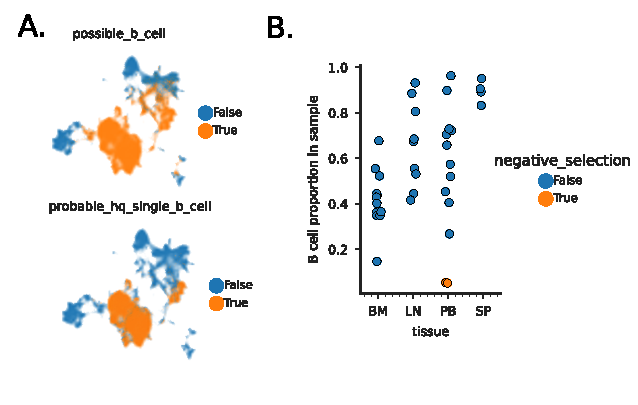
\includegraphics[width=\textwidth]{figs/Tabula_Bursa/SI/SI_Bpurifi.pdf}
    \caption{Physical and Computational Non-B cell removal}{(A) UMAP projections colored by whether cells are thought to be single B cells based on flags from \Section{sec:doublet-annotation}. Top represents every cell that \verb|celltypist| labels as a B cell (including many doublets), bottom shows the result of the doublet flagging methods described in the doublet detection section (B) Total proportion of B cells in all samples colored by whether or not negative selection was performed}
    \label{fig:B-filtering}
\end{figure}

\subsection{Cell cycle assignment}

We used MKI67 as a marker of cell cycle status. However, we noted that in cell types we often did not detect MKI67, even in plasmablasts which are thought to be cycling(\Fig{fig:cell-cycle}A left). This is likely due to technical limitations in sensitivity via droplet-based RNA sequencing. Thus, we took advantage of the co-variation between cell cycle genes to generate a more sensitive cell-cycle classification. First we calculated the correlation coefficient of all genes with MKI67. The distribution of the correlation values had a long tail of hundreds of genes with high ($> 0.5$) correlations. Manual inspection of the available evidence for the functions of these genes showed they were mostly involved in the G2/S phases cell cycle. We then used the top 30 most correlated genes to as a set create a cell cycle score using \verb|sc.tl.score_genes()| (\Fig{fig:cell-cycle}A right). Using a dataset of cycling B cells\cite{swift2023lineage}, we validated a threshold for calling cycling B cells as sensitive and specific(\Fig{fig:cell-cycle}B and C).  
\begin{figure}[h!]
    \centering
    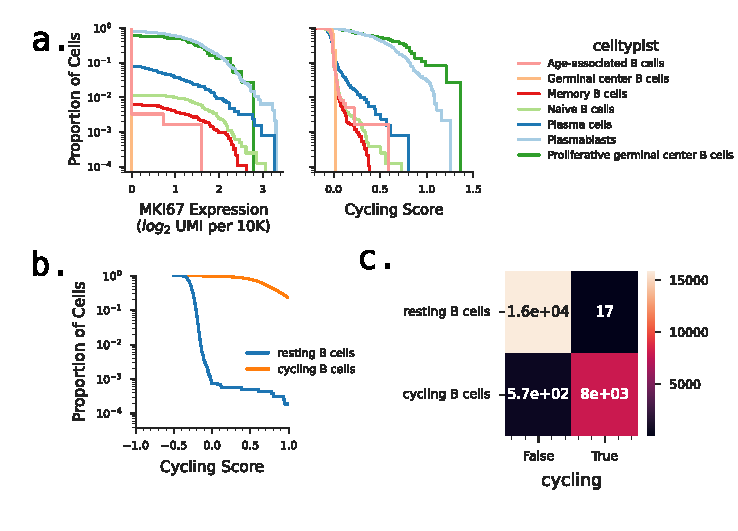
\includegraphics[width=\textwidth]{figs/Tabula_Bursa/SI/CellCycleSI.pdf}
    \caption{Cell Cycle Annotation}{(A) Distributions of MKI67 expression and Cell Cycling scores colored by celltypist labels. (B) Distributions of Cell Cycling Scores for \textit{in vitro} cycling B cells and resting B cells. (C) Confusion matrix of the ability of cycling score to distinguish between cycling and non-cycling B cells from \cite{swift2023lineage} at a score cutoff of 0.01}
    \label{fig:cell-cycle}
\end{figure}

\subsection{VAE model training and batch alignment} 
We used scVI\cite{lopez2018deep} to build a model of gene expression for all cells in the dataset, as well as a smaller model for the celltypist-defined B-lineage. Both models performed batch correction slightly more effectively than other methods we explored (BBKNN, \cite{polanski2020bbknn}, at the expense of increased computation resources taken to train the models. For scVI, we used the default parameters of the model except we changed the number of latent dimensions to 30 and the number of layers to 2. For each model, we included a batch key which was the unique sample ID of each 10X lane (``sample\_uid''). We also explored the use of other batch variables like the Donor ID and the tissue of origin, which performed less correction but possibly trivial donor-specific differences were apparent even after dimensionality reduction (e.g. XIST expression). We trained additional scVI models which added nuisance genes such as the top cell cycle genes, IGH genes, known tissue dissociation genes. We then used the latent representations of cells as the input for the Scanpy clustering methods (\verb|sc.pp.neighbors(adata, use_rep=``X_scvi”|). 

\subsection{Classification of high-quality B cell types and non-B cell types}
Our B cell enrichment was performed via negative selection on all samples besides the lymph nodes, which are often more than 30\% B cells. While this approach afforded an essentially unbiased look at the relative abundances of different B cells, it resulted in a relatively impure product particularly in bone marrow samples (\ref{fig:B-filtering}B). We noted that many of the contaminants were progenitor hematopoietic cells (~17\%) that likely escaped negative selection because of lower expression of their lineage markers. 

\subsection{Fine-grained annotation of B cell subtypes}
High-quality single B cells were separated into Memory, Antibody Secreting Cell, and Naive types using the \verb|Immune_All_Low| model and analyzed separately. While we explored a variety ways to analyze these gene expression profiles, ultimately we used the scVI representation to construct nearest-neighbors graphs (\verb|sc.pp.neighbors|), which were clustered using the Leiden algorithm at resolutions between 0.2 and 2 (\verb|sc.pp.leiden|). Guided by the dendrogram calculated for clusters (\verb|sc.tl.dendrogram|), we collapsed highly-similar clusters. For memory B cells, we incorporated antibody constant region information from the VDJ sequencing data. We classified cells as being switched (SW) if their assembly was not IGHM or IGHD, and non-switched (NS) otherwise. For antibody secreting cells, we used the scVI representation in which we had regressed MKI67 as a nuisance gene (\verb|X_scVI_cellcycle|) to cluster cells, which collapsed the distinction in the nearest-neighbors graphs between a particular cluster of Plasmablasts and Plasma cells. 


\section{VDJ sequence analysis and cell calling}
\subsection{VDJ sequence preprocessing}
\label{sec:vdj_preprocessing}
\noindent We used \verb|cellranger v7.0.1| to filter, trim and assemble VDJ reads into contigs. Our study design included both high-density loading of the VDJ-only samples and highly variable VDJ expression in certain tissues, and we found that both of these can lead to overly aggressive filtering by the default \verb|cellranger| VDJ annotation and cell-calling algorithm,  which is designed with a very low tolerance for doublets. Since the focus of our study prioritizes VDJ detection in VDJ-only samples over the default standard of removal of all probable doublet droplets, we designed a custom pipeline to replace the default \verb|cellranger| VDJ algorithm for contig annotation and cell calling. This allowed us to include all high-quality VDJ sequences in the analysis, while employing more stringent filtering on samples with paired gene expression data, as described below.

We used \verb|IgBLAST v1.17.0| to annotate all assembled contigs produced by \verb|cellranger| and further filtered the \verb|IgBLAST| output to retain only high quality, productive VDJ transcripts. Only contigs satisfying all of the following criteria were retained:
\begin{itemize}
    \item \verb|v_support| is less than $ \exp({-60})$,
    \item \verb|j_support| is less than $ \exp({-10})$,
    \item  V gene alignment is at least $ 160$ nucleotides long,
    \item  J gene alignment is at least $ 20$ nucleotides long,
    \item VDJ sequence is productive,
    \item VDJ sequence contains a CDR3,
    \item VDJ sequence contains no ambiguous bases.
\end{itemize}
For all purposes except for the providing evidence for the construction of the personalized V gene databases (see below), we further removed sequences that did not contain the full-length V gene (\verb|v_germline_start<=2|). We assigned these high quality VDJ sequences to lineages in a germline V gene reference-free way by performing single linkage clustering on sequences with the same same CDR3 length, and the same V gene family, and with the clustering condition requiring that the neither the fractional Hamming distance between the CDR3 nucleotide sequences nor the fractional Levenshtein distance between the templated regions exceeds $0.15$.

We then constructed a personalized germline V gene database for each donor using \verb|grmlin|, and re-annotated the contigs by aligning them to this personalized V gene database using \verb|BLAST v2.7.1| with the following additional options: \newline \verb|     -word_size 9 -dust no |\verb|-penalty -1 -gapopen 3 -gapextend 2|. \hfill \\ 

By comparing the germline allele assignments found by \verb|grmlin| and the germline assignments obtained by aligning the V sequence to the full IMGT database, we noticed that, in certain donors, there still remained a small number of likely germline alleles that remained undetected by \verb|grmlin|. These were V genes that were found in their unhypermutated form in several lineages and did not represent hypermutations of other V genes in the personalized V gene database. For each donor, we ranked such additional candidate germline genes by the distance to the most similar gene in the personalized database, and then by the number of lineages the unhypermutated version of the gene was associated with. Since each of these candidate germline genes can be associated with it's closest and, by construction, more highly expressed gene in the germline database, we further calculated the ratio, $r$, of lineages associated with each of these genes. We then iteratively added these candidate germline genes to a refined germline database if all of the following conditions were satisfied:
\begin{enumerate}
    \item the gene is supported by at least 5 lineages, OR is at least 5 mutations away from the closest germline gene in the database, and
    \item the ratio, $r$, exceeds $0.3/d_\mathrm{nearest}$, where $d_\mathrm{nearest}$ is the Levenshtein distance between these two genes.
\end{enumerate}


\subsection{Cell calling, V-gene tree construction, and detection and removal of cross-contaminants}

\subsubsection{Cell calling}
\label{sec:cell-calling}
\noindent A significant challenge of interpreting droplet-based single-cell experiment VDJ sequencing data is distinguishing between true cells and ambient transcripts. Specifically, because there is minimal separation between cell lysis and droplet generation, a large number of transcripts are released into the ambient prior to the encapsulation of individual cells. Distinguishing ambient VDJ transcripts from those associated with encapsulated cells becomes challenging, especially in light of the enormous variability in VDJ expression between antibody-secreting cells and naive and memory B cells, which can differ by more than two orders of magnitude (see \Section{sec:GEX-VDJ-merge} below). As a result, in the absence of gene expression data, it is in principle very difficult to distinguish between ambient and cell-associated VDJ transcripts. 

Since one of the main quantities of interest in our study are the patterns of co-variation in the presence of different VDJs in different tissues, we employ a permissive approach to calling VDJ ``cells" from this data, that we make more stringent in samples for which we do have gene expression data. Our approach has been designed with both long-read sequencing data applications (e.g. via the Pacbio platform), as well as reconstructed contigs of enzymatically fragmented amplicons (which, due to throughput limitations in long-read sequencing at the time of writing, is the exclusive source we use here, reconstructed by \verb|cellranger|, see \Section{sec:vdj_preprocessing} above). We begin by verifying that all contigs are either associated with a whitelisted 10X cell barcode, or within 1 nucleotide of an single whitelisted 10X barcode. We further discard all contigs supported by only a single UMI.

We then proceeded to assign these contigs to possible cells by iterating through all droplets and deriving a limited number of consensus contigs for each immunoglobulin locus (IGH, IGK, or IGL) using the approach described in the remainder of this section. In droplets that contained a unique VDJ per locus supported by multiple UMIs, we simply retained this contig, labeling it as a potential cell. However, as anticipated in droplet-based single cell experiments, a fraction of droplets in all samples contained contigs of the same chain that had multiple distinct VDJ sequences. These could either represent multiple encapsulated cells, ambient contaminants, or uncorrected reverse transcription, PCR or sequencing errors. 

To account for uncorrected errors arising in the library generation process, we first attempted to error-correct these sequences by deriving consensus sequences for each group of closely related VDJs. We did this by first constructing a minimum spanning tree for the VDJs associated with each immunoglobulin chain. We examined the the distribution of distances between adjacent sequences in the minimum spanning tree, and found that it typically had a very rapid decay at small distances, and a small number of edges connecting very distant VDJs. This distribution is consistent with a small number of distinct, true VDJs surrounded by rare variants arising through errors in the library generation or sequencing process. Motivated by this observation, the minimum spanning tree was then cut by removing all edges longer than 10 nucleotides. Thus, in each droplet, for each chain, we then had a collection of graphs representing connected components of VDJ sequences which likely only differed  due to library generation errors. We assigned a consensus sequence to each of these connected components via parsimony: we chose the VDJ sequence within the component that would require the smallest number of total library generation errors to explain the presence of closely-related variants.

Thus, we reduced the contigs associated with each droplet to a small number of consensus VDJ sequences that either represented multiple encapsulated cells, ambient contaminants, or a combination of the two types of species. We reasoned that ambient contaminants were likely to be supported with a smaller number of unique molecules than true cell-associated VDJs. Thus, in droplets in which there were multiple VDJs of this type, we only retained VDJs supported by at least 4 UMIs and that accounted for no fewer than 10\% of all the UMIs associated with that droplet. All other VDJs were designated ``ambient". 

Finally, we assigned a consensus C-gene call to each non-ambient VDJ. Due to sequence similarity among the different heavy chain isotypes, we found that, in a small fraction of cases multiple IGHC genes were associated with the same VDJ sequence in a cell. In these cases, we assigned the VDJ sequence the C-gene supported with the largest number of UMIs when that number was at least twice the number of UMIs supporting the second-ranked C-gene, and otherwise labeled the isotype as ambiguous.

\subsubsection{Construction of V-gene trees}
\noindent To construct phylogenetic trees of non-ambient templated V sequences within a lineage, we used \verb|MUSCLE v5.1| to first construct MSAs of all unique V nucleotide sequences within the lineage. In cases when the germline version of the gene was not present in the lineage (i.e. we did not sample a naive B cell from that lineage), we also added the germline version of the most common V gene call within that lineage to the MSA, which later allowed us to root the V gene phylogenies on this sequence. We used \verb|fasttree v2.1.11| to infer approximate maximum-likelihood phylogenies from these nucleotide MSAs, using the generalized time-reversible nucleotide evolution model and default parameters. 

\subsubsection{Detection and removal of cross-contaminants}

\begin{figure}[h]
    \centering
    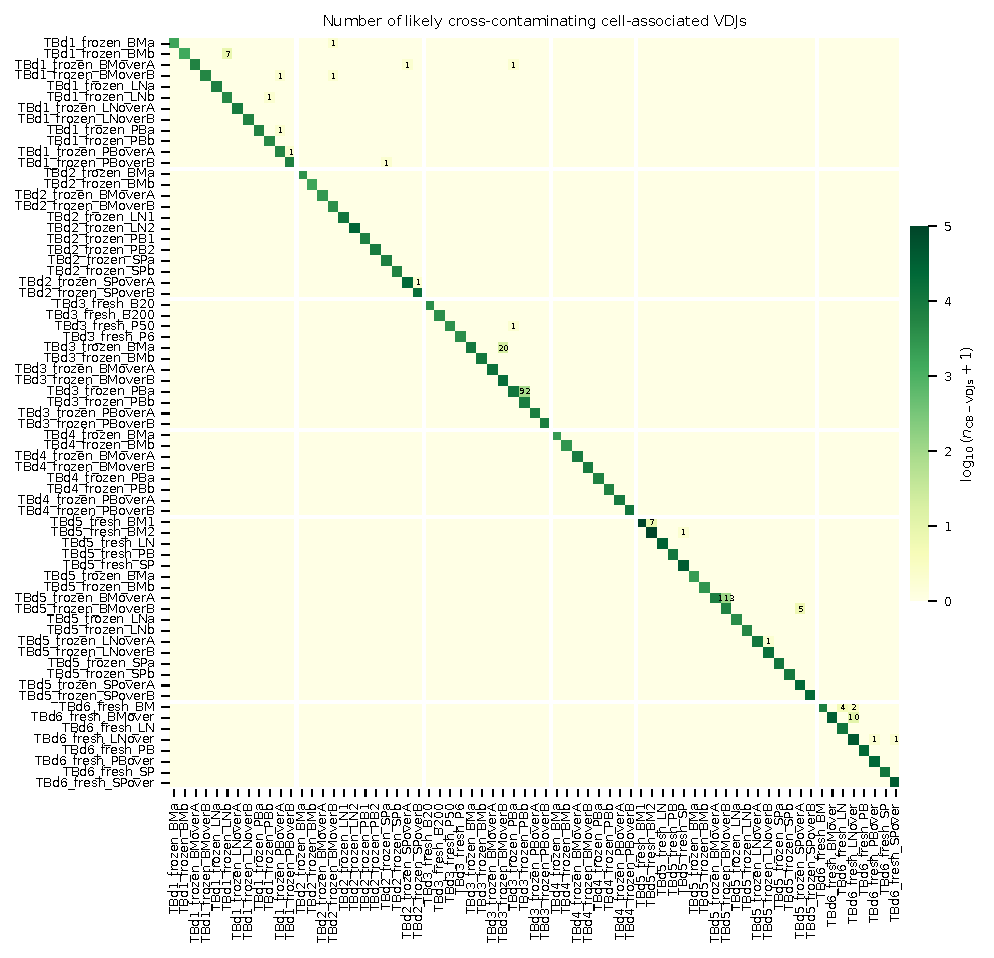
\includegraphics[width=\textwidth]{figs/Tabula_Bursa/SI/IGH_cross_contaminants_heatmap.pdf}
    \caption{Distribution of putative cross-contaminating heavy chains.}{Heatmap is colored by the logarithm of the total number of likely cross-contaminating cell barcode-VDJs for each pair of samples, and by the logarithm of the total number of private cell barcode-VDJs on the diagonal. The off-diagonal elements are annotated with the number of putative cross-contaminating VDJs.}
    \label{fig:IGH-cb_collision_numbers}
\end{figure}
\noindent Since the parallel preparation of several dozen libraries always carries the risk of cross-contamination, we endeavored to remove all potential cross-contaminating reads prior to downstream analysis. To detect cross-contamination events, we exploited the enormous diversity of both heavy chain VDJ nucleotide sequences and of 10X cell barcodes. We reasoned that, though we anticipate that we expect that multiple samples may contain either the same VDJ molecule or the same cell barcode, it is very unlikely that a VDJ shared between to samples is also associated with the same cell barcode. Specifically, given that we typically observe on the order of 100 shared VDJs even in replicates of the same tissue, and that there are about 737,280 possible cell barcodes by 10X design, the probability that there are any accidental collisions between any given pair of samples is on the order of $6 \times 10^{-3}$. Note that this still means that rare collisions are expected to occur in donors for which we have many samples of the same tissue, but that these collisions are expected to be rare, and that their removal should not significantly affect our estimates of rates at which sharing between tissues occurs.

Of the 1,024,568 unique cell barcode-VDJs in our dataset, we found 275 that were shared between multiple libraries (See \Fig{fig:IGH-cb_collision_numbers}). In all instances, this sharing occurred between pairs of samples from the same donor or pairs of samples that that were adjacent at some point in the library preparation procedure. The shared cell barcode-VDJs were typically associated with an overall very large number of UMIs that were typically concentrated in one of the samples (\Fig{fig:cross-contaminants-umi-ratio}), indicating that they likely originate from antibody-secreting cells and identifying one of the samples as the likely source of the contamination event. A small fraction of shared cell-barcode VDJs were associated with a very small number of total UMIs and/or were more evenly distributed among the pair of samples (\Fig{fig:cross-contaminants-umi-ratio}). These may represent true chance collisions of the cell barcode-VDJ pair, or may also be attributable to cross-contamination events but without a clear source sample. In this case, we removed the cell barcode-VDJ pair from further consideration. Conversely, when the shared cell barcode-VDJ was associated with a total of more than 100 UMIs, and when the fraction of UMIs in the secondary sample was smaller than $10^{-2}$, we removed the pair from the secondary sample and labeled the primary sample as the ``source" of the contamination event.

Given that shared cell barcode-VDJs were enriched for high-UMI-count VDJs when compared to cell barcode-VDJs that were private to one of the samples (\Fig{fig:cross-contaminants-umi-abundance}), we wanted to investigate whether there might also be a large number of undetected cross-contamination events affecting low-UMI-count cell barcode-VDJs. Specifically, since most VDJs are associated with few recovered heavy chain UMIs per cell, we were concerned that the transfer of a small number of those molecules between samples might lead to the association of that VDJ with the incorrect sample. To quantify the expected number of cross-contamination events affecting low-UMI-count VDJs, we constructed a simple model of the contamination process. Assuming that each UMI has an equivalent probability $\mu$ of being transferred between a pair of samples that can be involved in a cross-contamination event, the probability of a cell barcode-VDJ with $n$ total UMIs being transferred between two samples (and passing filtration, which requires at least 2 UMIs to be transferred.
Since cross-contamination can only occur between pairs of samples that are in physical proximity, to remain conservative, we limit the estimation of $\mu$ and $N_\mathrm{cont}(n)$ to samples in which we have identified pairs of shared cell barcode-VDJs. We estimate $\mu$ to be equal to the ratio of the sum of secondary-sample-UMIs associated with shared cell barcode-VDJs and all of the UMIs present in the pair of samples, which yields a probability of transfer per UMI of $\approx 4.5 \times 10^{-5}$. Plugging into our equation for cross-contamination, and plotting the result on \Fig{fig:cross-contaminants-umi-abundance}, we find that our model estimates that cross-contamination events involving cells with a small number of UMIs should be extremely unlikely. Thus, we conclude that many of the low-UMI-count contamination events may indeed represent chance collisions of cell-barcodes between samples that contain identical VDJs, but that these VDJs represent such a small fraction of the sampled VDJs that they are unlikely to affect our results.

\begin{figure}[t]
    \centering
    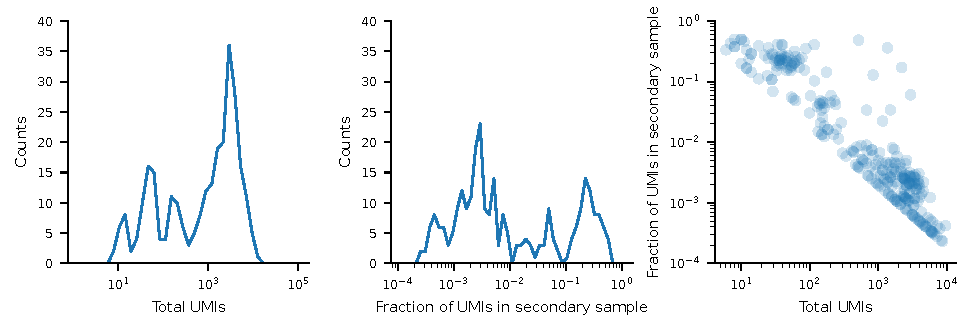
\includegraphics[width=\textwidth]{figs/Tabula_Bursa/SI/IGH_cross_contaminants_umi_ratio.pdf}
    \caption{Distribution of putative cross-contaminating heavy chains among the pair of samples between which they are shared}{(Left) Distribution of the total number of UMIs associated with the shared cell barcode-VDJ across the pair of samples. (Center) Distribution of the fraction of UMIs found in the sample with the smaller number of UMIs belonging to the cell barcode-VDJ pair. (Right) Scatterplot showing the two quantities for each shared cell barcode-VDJ event.}
    \label{fig:cross-contaminants-umi-ratio}
\end{figure}

\begin{figure}[t]
    \centering
    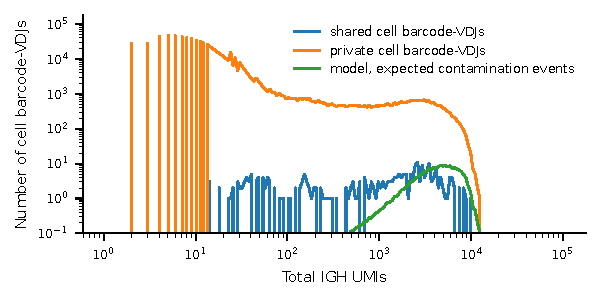
\includegraphics[width=4in]{figs/Tabula_Bursa/SI/IGH_cross_contaminants_vs_not_expression_with_pred.pdf}
    \caption{Heavy chain UMI abundance among shared cell barcode-VDJs and private cell barcode-VDJs among samples involved in any shared cell barcode-VDJ events.}{}
    \label{fig:cross-contaminants-umi-abundance}
\end{figure}

\subsection{Transcriptome-informed analysis and annotation of ambient transcripts}
\label{sec:GEX-VDJ-merge}
\noindent 

\section{Analysis of heavy chain sharing between donors}
\noindent VDJ nucleotide sequence sharing between donors is remarkably rare (5 in over 600 000 unique VDJ sequences, which justifies our use of the VDJ nucleotide sequence as a unique clonal identifier within a donor. When VDJs that are shared between donors do arise, they are always seen in cells in which we do not see any hypermutations in the templated V sequence. This suggests that are associated with commonly generated CDR3s arising in independent recombination events, as opposed to convergently evolved antibodies arising in response to a common antigen. Notably, the absence of shared  hypermutated VDJ nucleotide sequences suggests that even convergent recombination is far too rare an occurrence compared to the diversifying force of hypermutation to lead to the repeated generation of the identical heavy chain nucleotide sequence within the same individual. Note that this definition departs from the more commonly used definition of a ``clonotype'' (for heavy chains with an identical V-gene, J-gene and CDR3 amino acid sequence \cite{soto2019high}, and that it represents a far more stringent clonal identifier.

To verify that our shared VDJ nucleotides sequences indeed represent convergent recombinants in naive cells, we used OLGA to calculate CDR3 generation probabilities for all CDR3s associated with unhypermutated V-gene segments\cite{sethna2019olga}. Since the calculation of generation probabilities of hypermutated CDR3s also requires a model of hypermutation and selection in the germinal center reaction, which is not currently known in full, we further removed from consideration (for the purposes of this Section) all lineages in which we identified multiple unique CDR3 nucleotide sequences associated with unhypermutated VDJs. These species certainly contain hypermutated CDR3, and would lead to the erroneous inference of the generation probabilities for that CDR3, possibly skewing the entire distribution towards lower-probability CDR3's. As we show in , CDR3s found in a single donor have a wide variation of generation probabilities, as inferred by OLGA. In contrast, CDR3s associated with multiple donors have exceptionally high generation probabilities, as do CDR3s associated with the 5 instances of shared VDJ nucleotide sequences between donors. 

We calculated how our sharing statistics compare to those predicted by this empirical distribution of generation probabilities. To do this, we broadly followed the approach from Ref. \cite{elhanati2018sharing}, but with a slight departure in our enumeration of the number of independently generated CDR3s in our dataset. In Ref. \cite{elhanati2018sharing}, the authors, dealing with bulk TCR sequencing data, take the number of unique CDR3 amino acid sequences as a proxy for the number of unique recombination events. Here, we take the number of lineages associated with unique CDR3 nucleotide sequences and unhypermutated V genes to be the number relevant number independent rearrangements. We compare our sharing statistics to two versions of the sharing model, as in Ref. \cite{elhanati2018sharing}. First we calculated the expected amount of sharing assuming that the probability that a productive CDR3 sequence passes negative selection at the pre-B cell stage to be order $1$ (see dashed line, \textbf{Extended Data Figure 3e}). We find that this results in comparable, but slightly lower levels of sharing than seen in our data. Therefore, we concluded that it is likely that a much smaller percentage of productive CDR3's support high-enough quality antibodies to pass negative selection. This observation is consistent with a similar effect seen for TCRs, where only 3.7\% of all productive CDR3s pass thymic selection \cite{elhanati2018sharing}. Thus, we used our data to estimate an analogous ``selection factor" for B cells, by fitting the total number of unique amino acid CDR3 sequences, conditioned on the total number of sampled independent recombination events (lineages) in each donor. We find that this factor is variable among donors, likely reflecting the paucity of data for this type of estimation, but using the mean inferred selection factor of $1.8\%$, we find that the empirical number of shared CDR3s lies between the two extremes of the two models we considered.

\section{Data and code availability}

Raw sequencing reads will be deposited in the NCBI BioProject database upon publication. All associated metadata, as well as the source code for the raw data processing pipeline, downstream analyses, and figure generation, will be made available at GitHub upon acceptance. Processed AnnData objects will be available on the CellxGene Portal pending acceptance. 